\documentclass[a4paper,11pt,oneside,openany]{jsarticle}
\usepackage[dvipdfmx]{graphicx}
\usepackage{amsmath,amssymb}
\usepackage{bm}
\usepackage{graphicx}
\usepackage{ascmac}

\thispagestyle{empty}
%
\begin{document}
\begin{center}

  \vspace*{35mm}
  \huge 計算機科学実験及演習3 \par
  9班CPU\ ユーザーズマニュアル\\
  \vspace{90mm}
  \Large 提出期限:2019/6/14\\
   提出日: \today \\
  \vspace{15mm}
  \Large グループ番号: 9    \\
   1029293806\hspace{5mm}大山 偉永\par
   1029286786\hspace{5mm}富村 勇貴\par

  \vspace{10mm}
\end{center}
\clearpage
\addtocounter{page}{-1}

\newpage

\section{はじめに}
このPDFは京都大学工学部情報学科計算機科学コース2019年度前期木曜3,4,5限、金曜1,2,3,4,5限の計算機科学実験3で我々9班が作成したCPUのユーザーズマニュアルである。約一ヶ月半での作成期間であり多くの拡張機能を持つわけではなく性能が高いということはできないが最低限の命令は実行することができる。以下その具体的なマニュアルである。

\section{基本使用}
\begin{description}
  \item[完\,成\,日] 2019/5/30
  \item[コア数] 1
  \item[スレッド数] 1
  \item[FMAX] 74MHz
  \item[ワードサイズ] 16bit
  \item[メモリサイズ] 8,102B (4,096word $\times$ 2B)
\end{description}

\section{マイクロアーキテクチャ}
9班CPUはハーバードアーキテクチャとなっておりユーザーはデータメモリにデータを、命令メモリに命令を格納する必要がある。いづれも1word:16bitで4096wordまで格納可能で命令列については次項を参照。また汎用レジスタは8つ備えており、r[0], r[1],$\cdot\cdot\cdot$, r[7] と表記される。演算のソース/デスティネーションや主記憶のアドレス計算に用いられそのように命令のなかで使用する。アドレスについては変換などは行なわず、命令で定められるアドレスをそのまま主記憶のアドレスとする。またこの主記憶は、FPGA上に搭載されているRAMにて構成する。またIN、OUT命令についてはPowerMedusa MU500-RX/RK/7SEG上の8ビットDIPスイッチ二個をつなげて16bitの値を入力する。出力についてはLED:A0-A15を用いて16bitの値の出力を確認できる。
またreset命令はテンキースイッチのSW4を割り当てた。ユーザーはこのスイッチを押すことで命令をはじめからやり直すことができる。また電源が入った時点でも自動的にresetされるようになっている。このresetではプログラムカウンタの値は0になりレジスタの値も0に初期化されるがメモリの中身までは初期化できないのでユーザーはそこに注意する必要がある。さらにexec信号には同様にテンキースイッチのSW5を割り当てそれをおすことで命令を一時停止することができる。一度押すと命令の実行が一時停止されもう一度押すと再びそこから実行が再開される。

\newpage



\section{命令セットアーキテクチャ}
9班CPUには4種類の命令形式があり各命令形式とフィールドの意味は以下の通りである。ユーザーは以下の定義に従って16bitの命令列を命令メモリに格納することで命令が実行される。


\subsection{演算/入出力命令}
\begin{itemize}
  \item $I_{15:14} (op1) $. . . . . .操作コード (11) (operation code, opcode)
  \item $I_{13:11} (Rs)$ . . . . . .ソース・レジスタ番号
  \item $I_{10:8} (Rd)$ . . . . . .  デスティネーション・レジスタ番号
  \item $I_{7:4} (op3) $. . . . . . . 操作コード (0000 - 1111)
  \item $I_{3:0} (d) $. . . . . . . .  シフト桁数
\end{itemize}
9班CPUの演算/入出力命令を図\ref{enzan}に示す。演算命令では結果に基づく条件コードが設定される。
\begin{enumerate}
  \item 算術演算\\
  レジスタ Rd と Rs の加算 (ADD: add) または減算 (SUB: subtract) の結果を Rd に格納し、条
  件コードを設定する。条件コード C には最上位ビットからの桁上げが設定される。
  \item  論理演算\\レジスタ Rd と Rs の、ビットごとの論理積 (AND: and)、 論理和 (OR: or)、または排他的論理
  和 (XOR: exclusive-or) の結果を Rd に格納し条件コードを設定する。但し条件コード C は
  演算結果に関わらず 0 となる。
  \item 比較演算 (CMP: compare)\\レジスタ Rd から Rs を減算し、結果に基づく条件コード設定のみを行なう。条件コード C に
  は最上位ビットからの桁上げが設定される。
  \item 移動演算 (MOV: move)\\レジスタ Rd に Rs の値を単に格納し、Rd の値に基づき条件コードを設定する。但し条件コー
  ド C は Rs の値に関わらず 0 となる。
  \item シフト演算\\レジスタ Rd の値を、以下のようにシフトした値を Rd に格納し、条件コードを設定する。
  \begin{itemize}
    \item SLL (shift left logical) . . . . . . . . 左論理シフト。左シフト後、空いた部分に 0 を入れる。
    \item SLR (shift left rotate) . . . . . . . . . 左循環シフト。左シフト後、空いた部分にシフト・
    アウトされたビット列を入れる。
    \item SRL (shift right logical) . . . . . . . 右論理シフト。右シフト後、空いた部分に 0 を入れる。
    \item SRA (shift right arithmetic) . . . 右算術シフト。右シフト後、空いた部分に符号ビットの値を入れる。
  \end{itemize}
  シフト桁数は即値 d (0 - 15) である。また条件コード C には、シフト桁数が 0 の時または
  SLR では 0 が、それ以外では最後にシフト・アウトされたビットの値が設定される。条件コー
  ド V は常に 0 が設定される。
  \item 入出力命令
  \begin{itemize}
    \item IN (input) . . . . . . スイッチなどの機器から入力した値をレジスタ Rd に格納する。
    \item OUT (output) . . . レジスタ Rs の値を 7SEG LED などの機器に出力する。
    \item HLT (halt) . . . . . . SIMPLE を停止させる。
  \end{itemize}
  なお “(reserved)” と記された命令は何の動作もせず、単に次の命令に移行する。
\end{enumerate}
\begin{figure}[h]
  \centering
  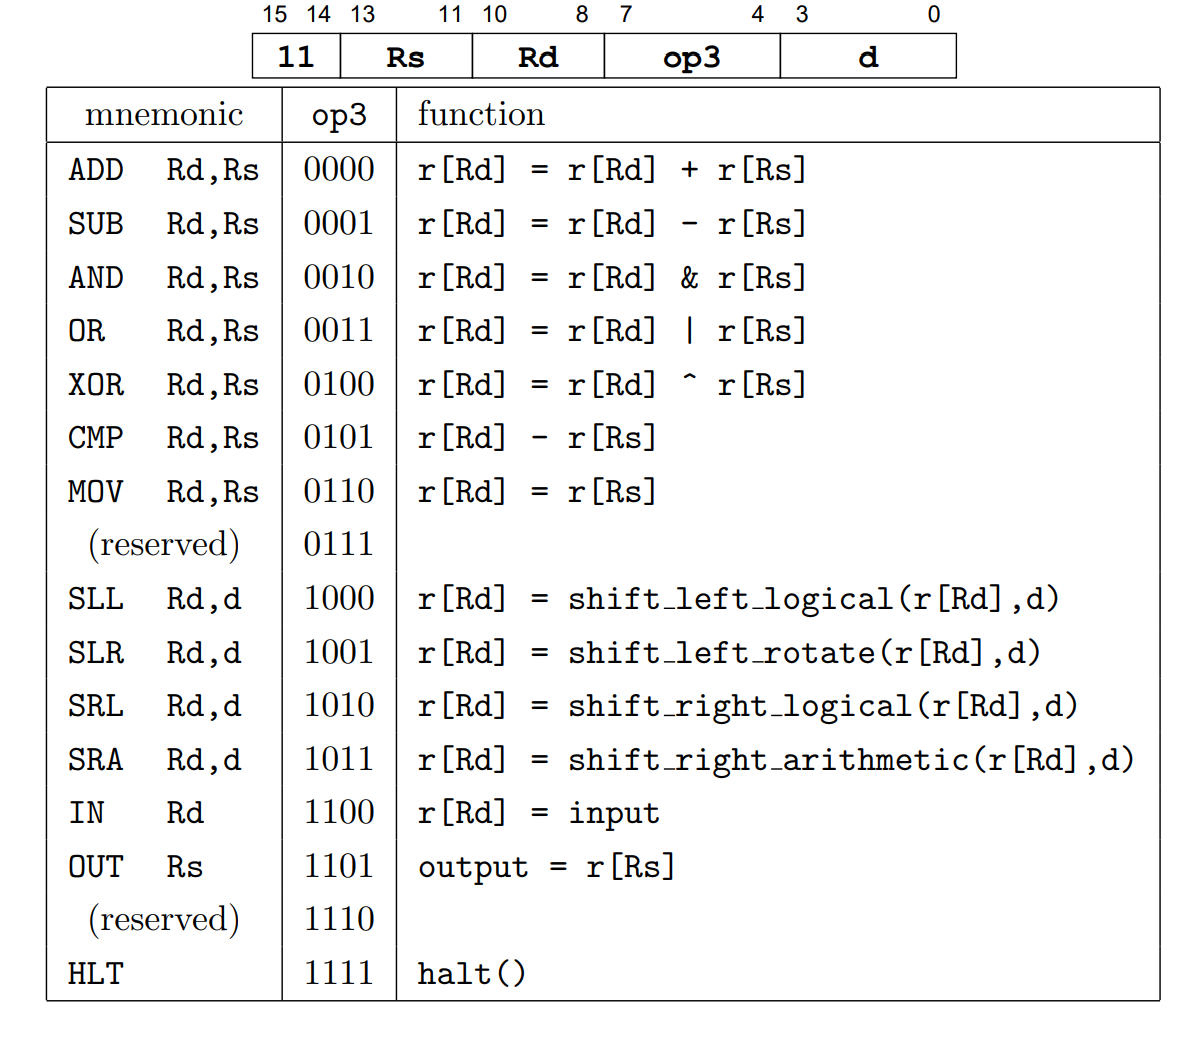
\includegraphics[width=10cm]{enzan.png}
  \caption{9班CPUの演算/入出力命令}
  \label{enzan}
\end{figure}



\subsection{ロード/ストア命令}
\begin{itemize}
\item $I_{15:14 }(op1)$ . . . . . 操作コード (00/01)
\item $I_{13:11} (Ra)$ . . . . . . ソース/デスティネーションのレジスタ番号
\item $I_{10:8} (Rb) $. . . . . . . ベース・レジスタ番号
\item $I_{7:0} (d)$ . . . . . . . . . 変位 (displacement)
\end{itemize}
9班CPUのロード命令 (LD: load) とストア命令 (ST: store) の機能を図\ref{load} に示す。ソース/デス
ティネーションは、フィールド Ra で指定されたレジスタ Ra である。また実効アドレスはベース・
レジスタ・アドレス指定により、フィールド Rb で指定されたレジスタ Rb と、フィールド d を符
号拡張した sign ext(d) を加算して求める。
\begin{figure}[h]
  \centering
  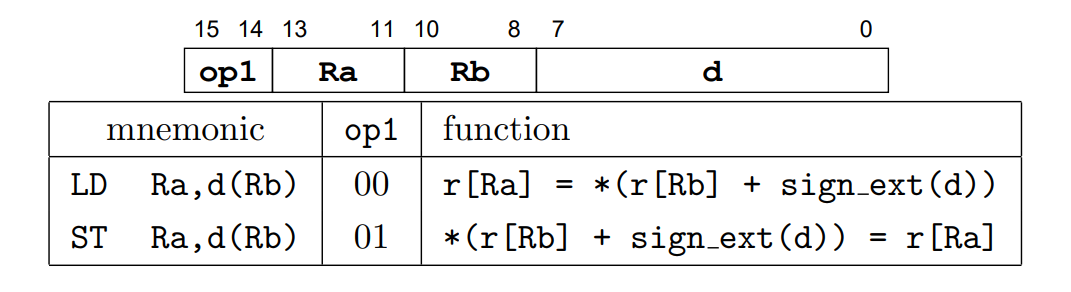
\includegraphics[width=10cm]{load.png}
  \caption{9班CPUのロード/ストア命令}
  \label{load}
\end{figure}


\subsection{即値ロード/即値演算/無条件分岐命令/ジャンプ命令}
\begin{itemize}
\item $I_{15:14} (op1)$ . . . . . 操作コード (10)
\item $I_{13:11} (op2)$ . . . . . 操作コード (000 - 110)
\item $I_{10:8} (Rb) $. . . . . . . ソース/デスティネーション/ベースのレジスタ番号
\item $I_{7:0} (d) $. . . . . . . . . 即値または変位
\end{itemize}
9班CPUの即値ロード命令 (LI: load immediate) 、即値加算命令(ADDI: add immediate)、ジャンプ命令(JMP: jump)、無条件分岐命令 (B: branch)、 即値比較命令(CMPI:compare immediate)の機能を図\ref{imm}
に示す。
\begin{itemize}
\item LI . . . . . 即値 sign ext(d) をレジスタ Rb に格納する。
\item ADDI . . . . 即値sign ext(d)とレジスタ Rbの値を加算しその結果をRdに格納し条件コードを設定する。
\item JMP . . . . .符号拡張したdの値をアドレスとしてPCのアドレス指定による分岐を行う。
\item B . . . . . . d を符号拡張した値を変位として、PC 相対アドレス指定による分岐を行なう。
\item CMPI . . . . .即値sign ext(d)とレジスタ Rbの値を比較しその結果をRdに格納し条件コードを設定する。
\end{itemize}
010 addi
011->jump
101 cmpi
\begin{figure}[h]
  \centering
  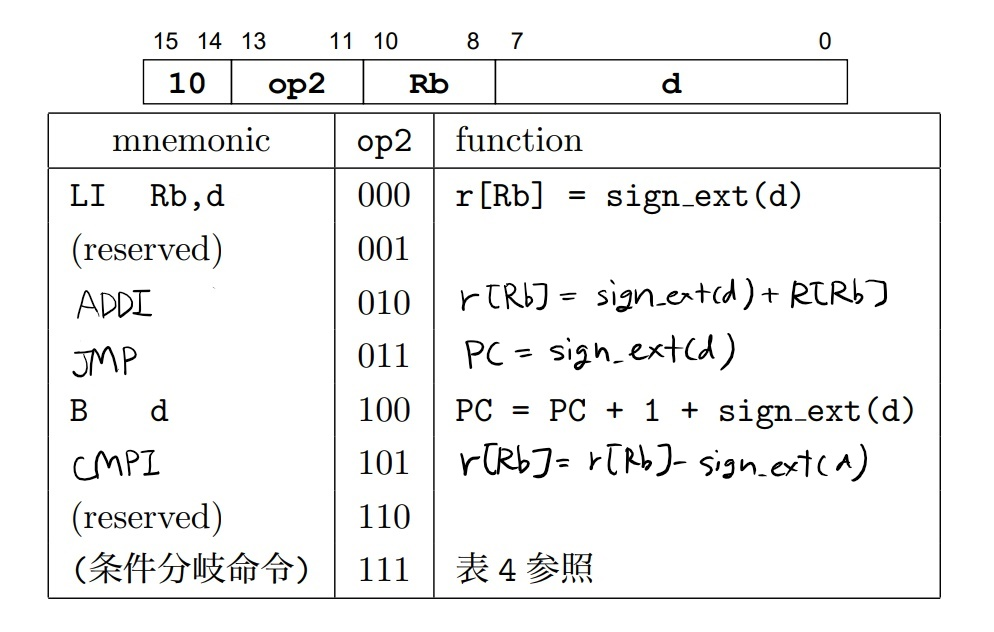
\includegraphics[width=10cm]{imm.jpg}
  \caption{9班CPUの即値ロード/即値演算/無条件分岐命令/ジャンプ命令}
  \label{imm}
\end{figure}



\subsection{条件分岐命令/nop命令}
\begin{itemize}
\item $I_{15:14 }(op1)$ . . . . . 操作コード (10)
\item $I_{13:11} (op2)$ . . . . . 操作コード (111)
\item $I_{10:8} (cond)$ . . . . . 分岐条件
\item $I_{7:0} (d)$ . . . . . . . . . 変位
\end{itemize}
9班CPUの条件分岐命令は図\ref{br}に示すように、フィールド cond で定められる分岐条件が成り立
てば PC 相対アドレスによる分岐、またはnop命令(何の動作もしない命令)を行ない、成り立たなければ単に次の命令に移行する。各命令の
分岐条件は以下の通り。
\begin{itemize}
\item BE (branch on equal-to) . . . . . . . . . . . . 条件コード Z が1
\item BLT (branch on less-than) . . . . . . . . . . 条件コード S と V の XOR(S\^\,V) が1
\item BLE (branch on less-than or equal-to) . . . Z または (S\^\,V) が1
\item BNE (branch on not-equal-to) . . . . . . . .  条件コード Zが0
\end{itemize}
\begin{figure}[h]
  \centering
  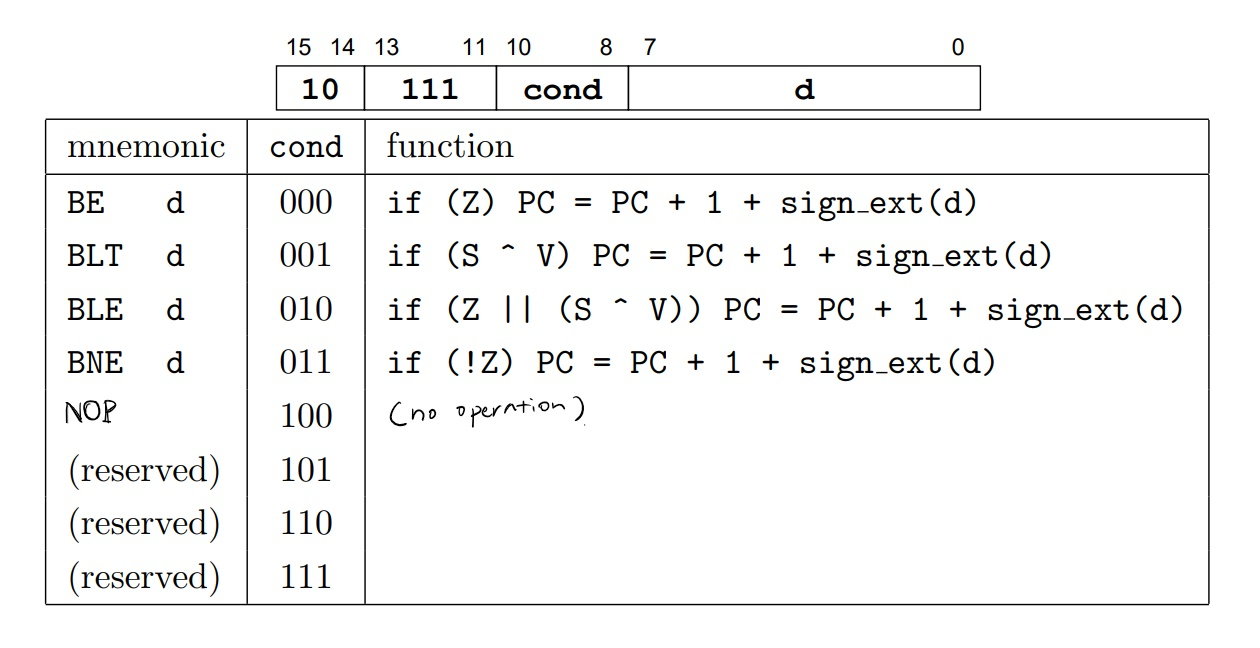
\includegraphics[width=10cm]{br.jpg}
  \caption{9班CPUの条件分岐命令}
  \label{br}
\end{figure}


\end{document}
